\section{Theory}

\subsection{Virtualization} 
\label{theory:virtualization}

In this section we are going to explain and show the differences between the two types of virtualization we have namely fullvirtualization and paravirtualization. The idea here is to give a short overview so the concept of each is understandable and to enable understanding of the suggested implementation. For a more comprehensive and detailed overview of these concepts please see the relevant references \footnote{ \href{https://www.vmware.com/content/dam/digitalmarketing/vmware/en/pdf/techpaper/VMware_paravirtualization.pdf}{Whitepaper regarding virtualization from VMWare}}

Virtualization is the concept of running software semi or fully isolated from the host system while giving the running software the impression it is running on a system of it’s own. Depending on the implementation the guest system (the virtualized environment) can also have direct or indirect access to the hardware. The host can section of parts of it’s system resources and give the guest full control over that hardware. It can also alternatively direct access to hardware through a hypervisor which will map the relevant full system the guest sees to the relevant allocated sections on the hosts system.

\subsubsection{Fullvirtualization}
\label{theory:fullvirtualization}

This type of virtualization is the most commonly used form of virtualization where all instructions executed on the guest goes directly to the hosts hardware. If the guest wishes to access any hardware like IO, memory or disk than it will trigger a trap into the hypervisor that is running underneath it all. A context switch will happen and the hypervisor handles the request of the guest system and returns what the guest would expect. This allows the hypervisor to for example store data that was supposed in the guest mind go to a physical hard disk in a file instead. The advantage of an approach like this is that you don’t need to make any changes to the guest system to make this work. You only need a precompiled executable and you can run it as long as the hypervisor is capable of handling all the relevant hardware requests. The disadvantage of this approach is that it’s a lot of overhead. Triggering a trap and context switch every time you need to access IO is very time consuming which is why fullvirtualization is a fair bit slower than running the software natively on the host.

\subsubsection{Paravirtalization}
\label{theory:paravirtualization}

In paravirtualization we have another and more effective approach to virtualization than fullvirtualization, although it is not without it’s downsides. Paravirtualization works in a similar way to fullvirtualization where we still abstract away hardware calls to a hypervisor which then handle these calls respectively. The change is that instead of going through a trap handler we recompile the respective guest system to call the respective hypervisor calls directly rather than making it think it’s accessing real hardware. In practice this might be implemented as syscalls to the hypervisor for the different types of hardware it wants to access. The advantage of this is that we get rid of the overhead by having a trap handler and needing to parse the respective hardware call in the hypervisor, making the hypervisor stage significantly faster. Though the disadvantage of this approach which might be obvious is that you need to recompile and change the running software todo this. This can be a time consuming endeavor since it requires familiarity with the code base to know which function that needs to be patched. Sometimes the source code is also not always available if the plan is to virtualize any proprietary software where you only have access to the binary files. Which makes the process of patching even more harder since you would need to reverse engineer and find the relevant function before patching them.

\begin{figure}[htbp]
    \centering
    %\includesvg[]{Images/Kernel_Layout.svg}
    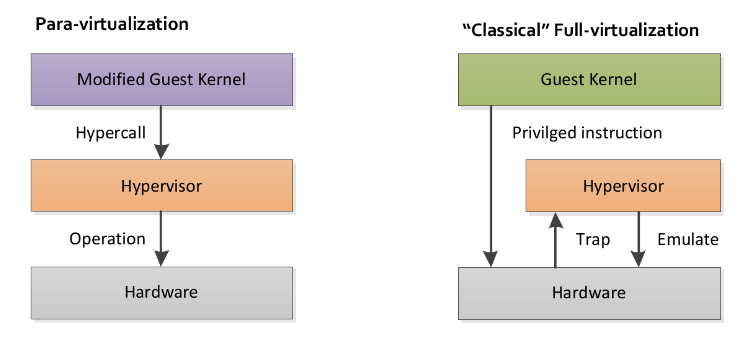
\includegraphics[width=\textwidth]{Images/Virtualization_-_Para_vs_Full.png}
    \caption{Full virtualization compered to paravirtualization}
    \figsource{RicoRico, CC BY-SA 4.0 (https://creativecommons.org/licenses/by-sa/4.0), via Wikimedia Commons}

    \label{fig:vir-para-vs-full}
\end{figure}

In the end what of these two virtualization methods are best really comes down to the problem you are trying to solve. For running many different types of software fullvirtualization might be the more ideal. If you are trying to virtualize specialized software you have familiarity with you can gain a lot by rewriting it to interact directly with the hypervisor

